\chapter{La rekursiveco}
{ }\hfill\textbf{Nivelo:} meza

\noindent  La lingvo Logo uzas tre ofte te^hnikon programadan nomatan
rekursiveco.  En ^ci tiu ^capitro, ni malkovros tuj tiun koncepton per
simplaj ekzemploj por poste profundi^gi per ^cefe la desegnado de
fraktalo nomata la ne^gero de Van Koch.  Por komenci, jen malgranda klarigo:
\begin{center}
\textbf{Proceduro estas rukursivo se ^gi vokas sin mem.}
\end{center}
\section{En desegnejo}
\subsection{Unua ekzemplo}
\begin{verbatim}
por ekz1
dn 1
ekz1
fino  
\end{verbatim}
Tiu proceduro estas rekursiva ^car la proceduro \texttt{ekz1} estas
vokata je la lasta linio.  Dum la rulado, oni konstatas ke la testudo
ne ^cesas turni^gi.  Por haltigi la programon, oni nepre premu la
butonon STOP.
\subsection{Dua ekzemplo}
\noindent Anta^u ^cio, jen tri novaj primitivoj:
\begin{itemize}
\item [$\bullet$] \texttt{atendu nombro}\hspace {4cm } \textcolor{red}{ \texttt{atendu 60}}\\
Haltigu la programon dum tiom da 60$^{\textrm{onoj}}$ de sekundo kiel indikite. \\
Ekzemple, \texttt{atendu 120} haltigos la programon dum du sekundoj.
\item [$\bullet$] \texttt{gum,gumskrapu}\hspace {4cm } \textcolor{red}{{gumskrapu}}\\
Kiam la testudo movi^gas, ^gi forvi^sas anstata^u skribi post si.
\item [$\bullet$] \texttt{desegne}\hspace {4cm } \textcolor{red}{{desegne}}\\
Metu la testudon en la moduson de klasika desegno: la testudo skribas post si dum movi^gi.
\end{itemize}
\noindent
\begin{verbatim}
por ekz2
an 200 gum atendu 60
man 200 desegne dn 6
ekz2
fino
\end{verbatim}
Nur restas ruli tiun programon.  Je ^ciu sekundo la sama motivo
rekomenci^gas kaj la programo ^sajnigas sekundhorlo^gon!
\section{En tekstejo}
\subsection{Unua ekzemplo}
\noindent La primitivo \texttt{skribu, s} ebligas skribi tekston en la
tekstareon.  ^Gi atendas kiel argumenton jen liston, jen vorton.  Ekz.:
\texttt{s "saluton} \texttt{s [Mi skribas kion mi volas]}.  (Ne
forgesu la citilon " kiam oni volas skribi nur vorton.)
\begin{verbatim}
por ekz3 :n
skribu :n
ekz3 :n+1
fino
\end{verbatim}
Rulu la komandon \texttt{ekz3 0}, poste haltigu per butono STOP.
Faru la ^san^gojn necesajn en tiu programo por ke la numeroj aperu duope.

Nun mi volas skribi ^ciun nombron pli grandan ol $100$ kiu estas en la
multipliktabelo de la kvino.  Sufi^cas do modifi la programon jene:
\begin{verbatim}
por ekz3 :n
skribu :n
ekz3 :n+5
fino
\end{verbatim}
kaj ruli: \texttt{ekz3 100}
\subsection{Realigi eliran provon}
\noindent Tajpu la jenajn komandojn:\\
\texttt{se 2+1=3 [skribu [tio estas vera]]} \\
\texttt{se 2+1=4 [skribu [tio estas vera]] [skribu [la kalkulo estas malvera]]} \\
\texttt{se 2+5=7 [s "vera] [s "malvera]}\\
\\
Se vi ankora^u ne komprenas la sintakson de la primitivo \texttt{se},
adresi^gu al la referenca gvidlibro \xlogo.
\begin{verbatim}
por ekz3 :n
se :n=100 [haltu]
skribu :n
ekz3 :n+1
fino
\end{verbatim}

Rulu la komandon \texttt{ekz3 0}

Faru la ^san^gojn necesajn en tiu programo por aperigi la nombrojn
ku^santaj inter $55$ kaj $350$ kiu estas en la multipliktabelo de la
dek-unuo.

\section{Ekzemplo de fraktalo: la ne^gero de Koch}

Danke al la rekursiveco, tre facilas generi en \logo\ objektojn
nomatajn en matematiko \emph{fraktaloj}.

Jen la unuaj stadioj ebligantaj krei la malglatan linion de Van Koch.
\begin{center}
  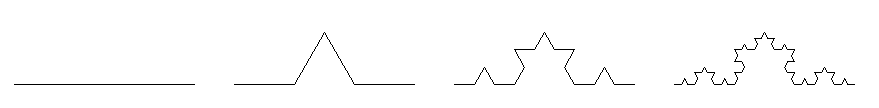
\includegraphics[width=\textwidth]{bildoj/koch0123.png}
\end{center}
En ^ciu stadio:
\begin{enumerate}
\item ^Ciu segmento estu partigita en tri egalajn partojn.
\item Oni grafiku egallateran trilateron sur la dua segmento.
\item Oni forigu tiun duan segmenton.
\end{enumerate}
\textbf{Rimarkenda:} Konsiduru la duan stadion; konstatu ke tiun
linion formas kvar motivoj rilataj al l' anta^ua stadio kaj kies
amplekso estas triono.  Tiel evidenti^gas la rekursiva naturo de la
fraktalo.

Nomu $L_{n,\ell}$ la motivon longa je $\ell$, grafikita en la stadio $n$.
Por grafiki tiun motivon jen la procedo:
\begin{enumerate}
 \item Desegnu $L_{n-1,\ell/3}$
 \item Turnu maldekstren je $60$ gradoj
 \item Desegnu $L_{n-1,\ell/3}$
 \item Turnu dekstren je $120$ gradoj.
 \item Desegnu $L_{n-1,\ell/3}$
 \item Turnu maldekstren je $60$ gradoj
 \item Desegnu $L_{n-1,\ell/3}$
\end{enumerate}
En \logo, tio fari^gas tutsimple:
\begin{verbatim}
# :l longo de la motivo 
# :p stadio
por linio :l :p
se :p=0 [an :l] 
  [linio :l/3 :p-1 dn 60 linio :l/3 :p-1 dn 120 linio :l/3 :p-1 dn 60 linio :l/3 :p-1]
fino
\end{verbatim}
Se oni desegnas egallateran trilateron konsistanta el tri tiaj linioj,
oni akiras mirindan ne^geron de Van Koch
\begin{verbatim}
# :l longo de la latero
por neĝero :l :p
ripetu 3 [linio :l :p dn 120]
fino
\end{verbatim}
Poste rulu: \texttt{flocon 200 6}
\begin{center}
  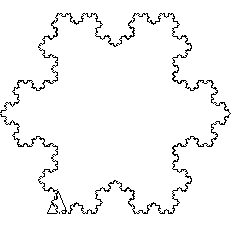
\includegraphics{bildoj/flocon.png}
\end{center}
\section{Rekursiveco pri vortoj}
Priser^cu la liston de primitivoj je p.\,\pageref{liste-prim} por
kompreni la rolon de la primitivoj \texttt{vort}, \texttt{lastan}, kaj
\texttt{senlastan}.

Jen rekursiva proceduro kiu ebligas renversi l' ordon de la literoj de
vorto.
\begin{verbatim}
por renversuv :v
se malplena? :v [sendu "]  
sendu vorton lastan :v renversuv senlastan :v
fino

skribu renversuv "abcĉde
edĉcba
\end{verbatim}
Oni diras ke vort' estas palindromo se oni povas legi ^gin je amba^u
direktoj (ekzemploj: ama, radar', onano...).
\begin{verbatim}
# testu ĉu la vorto :v estas palindromo
por palindromo :m
se  :m = renversuv :m [sendu vera] [sendu malvera] 
fino
\end{verbatim}
Kaj finfine jen mojosa programeto (dankon Olivier SC):
\begin{verbatim}
por palin :n
se palindromo :n [skribu :n haltu]
skribu (list :n "PLUS renversuv :n "EGALAS sumon :n renversuv :n)
palin :n + renversuv :n 
fino

palin 78
78 PLUS 87 EGALAS 165
165 PLUS 561 EGALAS 726
726 PLUS 627 EGALAS 1353
1353 PLUS 3531 EGALAS 4884
4884
\end{verbatim}
\section{Kalkuli faktorialon}
\label{factorielle}
Oni difinas faktorialon de $5$, indikite $5!$ jene:
 $$5!=5\times4\times3\times2\times1=120$$
^Generale, por $n$ strikte pozitiva, rimarku ke: $n!=n\times(n-1)!$.
Tiu rilato klarigas la rekursivan naturon de jena programo:
\begin{verbatim}
por fak :n
se :n=0 [snd 1] [snd :n * fak :n-1]
fino

s fak 5
120
s fak 6
720
\end{verbatim} 
 \section{Proksimumo de $\pi$}
\label{approx-pi}
Oni povas akiri proksimumon de la nombro $\pi$ per la formulo:
$$\pi\approx2^k\sqrt{2-\sqrt{2+\sqrt{2+\ldots\sqrt{2+\sqrt2}}}}$$ 
kie $k$ estas la nombro de kvadrataj radikoj.  Ju pli granda estas $k$
des pli tiu esprimo proksimi^gas al nombro $\pi$.

La formulo konsistas el la esprimo $2+\sqrt{2+\ldots\sqrt{2+\sqrt2}}$
kiu estas klare rekursiva, de kie la programo jena:
\begin{verbatim}
# k estas la nombro de radikoj
por aprokspi :k
tajpu "Proksimume:\  s (potencon 2 :k) * radikon (2 - radikon (kalk :k-2))
s "-------------------------
tajpu "Pi:\  s pi
fino

por kalk :p
se :p=0 [snd 2] [snd 2 + racine kalk :p-1]
fino

aprokspi 10
Proksimume: 3.141591421568446 
------------------------- 
Pi: 3.141592653589793 
\end{verbatim}
Oni akiris la $5$ unuajn decimalojn!  Se oni deziras pli, necesos
forigi kelkajn kalkulerarojn pro ne precize kalkuli la koncernitajn
kvadrataj radikojn.  Por tio ni pligrandigos la nombron de decimaloj
per la primitivo \texttt{decimalojn\_provizu}.
\begin{verbatim}
decimalojn_provizu 100
aprokspi 100
Proksimume: 3.1415926535897932384626433832795028841973393069670160975807684313880468...
------------------------- 
Pi: 3.141592653589793238462643383279502884197169399375105820974944592307816406....
\end{verbatim}
Kaj nun oni akiras 39 decimalojn...
